\chapter{Introduction}

\section {Domain overview}

\tab Software systems are continuously in change. As long as the software system is used the changing process is never finished. Changes can be triggered by new features, defects, new technologies, system refactoring for maintainability.\\ Software maintenance can be made during the development process by maintaining the already implemented features, while developing new ones or at the end of the development process when the system is no longer open to new features requested by the client and the maintenance is only made for the existing ones.\\

\tab During the development process of a software system new classes and new methods to the existing classes are added in order to fulfill new functionalities. All of the adding actions from above have a direct impact on the system structural dependencies. Those are the result of the source code analysis of the system. \\The source code is any static, textual, human readable, fully executable description of a computer program that can be compiled automatically into an executable form \cite{ct1}.\\On the other hand logical dependencies also can be added during the development process. Logical dependencies refer to those depencencies between entities that are not always visible through source code analysis. Logical dependencies can be easily extracted from the versioning system (e.g. Subversion , Git) commits.  (Figure \ref{fig:fig1}).

\tab The ideal situation presumes that changes in one part can be made without changing parts that are in a dependency relation with that part. Those dependencies affect the maintainability of the system and increase the realization effort of any problem that appears during the maintenance time. Studying only the structural dependencies of the system is not enough to get a clear overview of the system dependencies. For more precise results is needed a study that combines structural dependencies and logical dependencies. 


\begin{figure}[h]
\centering
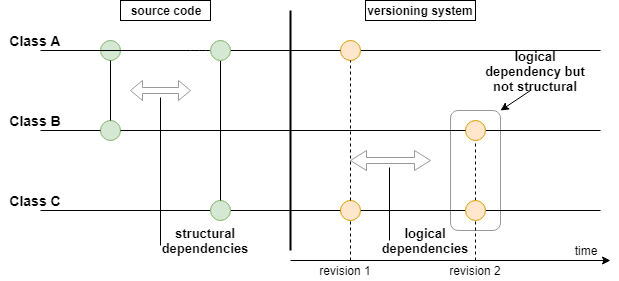
\includegraphics[scale=0.60]{fig1.png}
\caption{Relationships between structural and logical dependencies }
\label{fig:fig1}
\centering
\end{figure}

\section {Thesis objectives}
In this paper we intend to understand better the intersection between structural dependencies and logical dependencies and their impact over the system stability (Figure \ref{fig:fig2}). 

\begin{figure}[h]
\centering
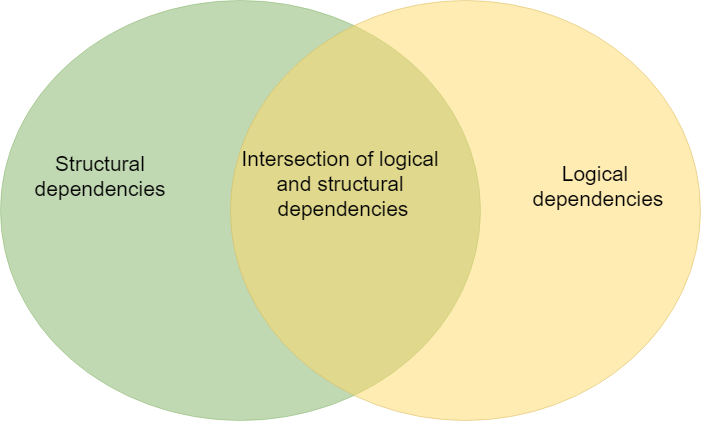
\includegraphics[scale=0.4]{fig2.png}
\caption{Venn Diagram showing the intersection between structural and logical dependencies }
\label{fig:fig2}
\end{figure}

\tab In earlier studies, the relationships between logical and structural dependencies have been analysed (Oliva and Gerosa, 2011 \cite{ct_oliva2011} ; Yu, 2007 \cite{ct5};  Oliva and Gerosa, 2015 \cite{ct6}, Cappiluppi and Ajienka, 2017 \cite{ct8},  Cappiluppi, Ajienka and Counsell, 2018 \cite{cappilupi2}). All of these studies showed that most of the structural dependencies do not co-evolve and a great part of logical dependencies are not doubled by structural dependencies.\\

\tab In this work we build logical dependencies based on three questions with related motivations presented in the following :

\textit{\textbf{Question 1}} . How the number of source files changed in a commit can influence the logical dependencies of the system and the overlapping rates with the structural dependencies.\\
\textit{Motivation} : A commit that has as participants a big number of files can indicate that a merge with another branch or a folder renaming has been made. In this case, a series of irrelevant logical dependencies can be introduced since not all the files are updated in the same time for a development reason. Because of this, Cappiluppi and Ajienka, in their works \cite{cappilupi2}, \cite{ct8} only take into consideration commits with less then 10 source code files changed in building the logical dependencies. But, on the other hand, sometimes large commits are unavoidable, e.g. a major change in API, so we will also study large commits but we will split the logical dependencies extracted into categories based on the number of files changed so that we can compare the impact of this sectioning on the final results.

\textit{\textbf{Question 2}}. Considering comments can lead to additional logical dependencies ? How many logical dependencies are introduced by considering comment changes as valid changes and in what percentage this can influence the final result ?\\
\textit{Motivation} : Not all the commits that have source code files changed include code changes , some of them can be only comments changes. Regarding this aspect, we can consider that there is no logical dependency between two classes that change in the same time only by comments changes . Some studies have not taken this aspect into consideration, so we will analyse the impact of not considering/ considering comments as valid changes on the results. 


\textit{\textbf{Question 3}}. One occurrence of a logical dependency is enough to consider it as valid ? If we consider only logical dependencies with more then one occurrence as valid, the results are influenced in a significant way ?\\
\textit{Motivation} : One occurrence of a logical dependency between two classes can be a valid logical dependency, but can also be a coincidence. Taking into consideration only logical dependencies with multiple occurances as valid dependencies can lead to more accurate logical dependencies and more accurate results.\\ But if the project studied has a relatively small amount of commits, the probablilty to find multiple updates of the same classes in the same time can be small, so filtering after the number of occurences can lead to filtering all the logical dependencies extracted. Giving the fact that we will study multiple projects of different sizes and number of commits, we will analyse also the impact of this filtering on different projects.\\

\tab In order to answer these research questions, we have built a tool that extracts structural and logical dependencies on different scenarios, the design and implementation of the tool is presented in chapters 3 and 4.\\
\tab We have analyzed 19 open-source software systems of different sizes within the tool developed, the experimental results obtained being presented in chapter 5 . The final chapter, chapter 6, discusses the conclusions drawn from our experimental 
research.

